\documentclass{book}
\usepackage{amsmath}
\usepackage{graphicx}
\usepackage{hyperref}
\usepackage{amssymb}
\usepackage{amsfonts}
\usepackage{tcolorbox}
\usepackage{hyperref}
\usepackage[latin1]{inputenc}
\graphicspath{ {./images/} }

\hypersetup{
    colorlinks=true,
    linkcolor=cyan,
    filecolor=magenta,      
    urlcolor=blue,
}

\title{Calculus Single Variable}
\author{Robert Ghrist}
\date{11/15/16}

\begin{document}
\boldmath
\maketitle

\tableofcontents{}

\begin{sloppypar}
\part{Calculus Single Variable}

\chapter{Functions} \label{ChFunctions}

\section{Functions} \label{ChFunctionsSecFunctions}

A \textit{function} can be visualized as a machine that takes in an input $x$ and returns an output $f(x)$. The collection of all possible inputs is called the \textit{domain}, and the collection of all possible outputs is called the \textit{range}.\\
This course deals with functions whose domains and ranges are $\mathbb{R}$ or subsets of $\mathbb{R}$ (this is the notation for the real numbers).\\\\
\textbf{Examples}
\begin{enumerate}
\item Polynomials, e.g. ${f(x) = x^3-5x^2+x+9}$. Give the domain and range of $f$.\\
Answer: The domain is $\mathbb{R}$, because we can plug in any real number into a polynomial. The range is $\mathbb{R}$, which we see by noting that this is a cubic function, so as ${x \rightarrow -\infty}$, ${f(x) \rightarrow -\infty}$, and as ${x \rightarrow \infty}$, ${f(x) \rightarrow \infty}$.
\item Trigonometric functions, e.g. $\sin$, $\cos$, $\tan$. Give the domain and range for each of these.\\
Answer: For $\sin$ and $\cos$: domain is $\mathbb{R}$; range is ${\left[-1,1\right]}$. For $\tan$, the domain is ${\lbrace x \in \mathbb{R}: x \neq \frac{\pi}{2}+k\pi\rbrace}$; range is $\mathbb{R}$.
\item The exponential function, $e^x$. Give the domain and range for the exponential.\\
Answer: Domain is $\mathbb{R}$; range is (${(0,\infty)}$.
\item The natural logarithm function, ${\ln x}$. Recall that this is the inverse of the exponential function. Give the domain and range for ${\ln x}$.\\
Answer: Domain is $(0,\infty)$; range is $\mathbb{R}$. Notice how the domain and range of the exponential relate to the domain and range of the natural logarithm.
\item Is ${\sin^{-1}}$ a function? If so, why? If not, is there a way to make it into a function?
\\Answer: ${\sin^{-1}}$ is not a function, because one input has many outputs. For example, ${\sin^{-1}(0) = 0,\pi,2\pi,\ldots}$. By restricting the range of ${\sin^{-1}}$ to ${\displaystyle\left[-\frac{\pi}{2},\frac{\pi}{2}\right]}$, one gets the function $\arcsin$.
\end{enumerate}

\subsection{Operations on Functions} \label{ChFunctionsSubsOperationsOnFunctions}

\textbf{Composition}\\
The \textit{composition} of two functions, $f$ and $g$, is defined to be the function that takes as its input x and returns as its output $g(x)$ fed into $f$.
\begin{equation*} f\circ g(x)=f(g(x)) \end{equation*}
\\
\textbf{Example:}\\
${\sqrt{1-x^{2}}}$ can be thought of as the composition of two functions, $f$ and $g$. If ${g=1-x^{2}}$, $f$ would be the function that takes an input $g(x)$ and returns its square root.\\\\
\textbf{Example:}\\
Compute the composition ${f \circ f}$, i.e. the composition of $f$ with itself, where ${\displaystyle f(x) = \frac{1}{x+1}}$.\\
Answer:\\
We find that
\begin{align*}
f \circ f(x)&=f(f(x))\\
&=f \left(\frac{1}{x+1}\right)\\
&=\frac{1}{1/\left(x+1\right)+1}\\
&=\frac{x+1}{1+x+1}\\
&=\frac{x+1}{x+2}.
\end{align*}
\\\\
\textbf{Inverse}\\
The \textit{inverse} is the function that undoes $f$. If you plug ${f(x)}$ into ${f^{-1}}$, you will get $x$. Notice that this function works both ways. If you plug ${f^{-1}(x)}$ into $f(x)$, you will get back $x$ again.
\begin{equation*} f^{-1}(f(x))=x \end{equation*} 
\begin{equation*} f(f^{-1}(x))=x \end{equation*}
NOTE: ${f^{-1}}$ denotes the inverse, not the reciprocal. ${f^{-1}(x)\neq\frac{1}{f(x)}}$.\\\\
\textbf{Example:}\\
Let's consider ${f(x)=x^{3}}$. Its inverse is ${f^{-1}(x)=x^{\frac{1}{3}}}$.
\begin{equation*} f^{-1}(f(x))=(x^{3})^{\frac{1}{3}}=x \end{equation*}
\begin{equation*} f(f^{-1}(x))=(x^{\frac{1}{3}})^{3}=x \end{equation*}
Notice that the graphs of $f$ and $f^{-1}$ are always going to be symmetric about the line ${y=x}$. That is the line where the input and the output are the same.

\subsection{Classes of Functions} \label{ChFunctionsSubsClassesOfFunctions}

\textbf{Polynomials}\\
A polynomial $P(x)$ is a function of the form 
\begin{equation*} P(x)=c_{0}+c_{1}x+c_{2}x^{2}+\dots+c_{n}x^{n} \end{equation*}
The top power $n$ is called the degree of the polynomial. We can also write a polynomial using a summation notation.
\begin{equation*} P(x)=\sum_{k=0}^{n}c_{k}x^{k} \end{equation*}\\
\textbf{Rational functions}\\
Rational functions are functions of the form ${\displaystyle\frac{P(x)}{Q(x)}}$ where each is a polynomial.\\\\
\textbf{Example:}\\
\begin{equation*} \displaystyle\frac{3x-1}{x^{2}+x-6} \end{equation*} is a rational function. You have to be careful of the denominator. When the denominator takes a value of zero, the function may not be well-defined.\\\\
\textbf{Powers}\\
Power functions are functions of the form ${cx^{n}}$, where $c$ and $n$ are constant real numbers.\\
Other powers besides those of positive integers are useful.\\\\
\textbf{Example:}\\
What is ${x^{0}}$ ?\\
Answer:\\
${x^{0}=1}$\\\\
What is ${x^{-\frac{1}{2}}}$ ?\\
Answer:\\
Recall a fractional power denotes root. For example, ${x^{\frac{1}{2}}=\sqrt{x}}$. The negative sign in the exponent means that we take the reciprocal. So, ${x^{-\frac{1}{2}}=\frac{1}{\sqrt{x}}}$.\\\\
What is ${x^\frac{22}{7}}$ ?\\
Answer:\\
One can rewrite this as ${\left(x^{22}\right)^{1/7}}$. That means we take $x$ to the 22nd power and then take the 7th root of the result.\\
${x^\frac{22}{7}=\sqrt[7]{x^{22}}}$\\\\
What is ${x^{\pi}}$ ? We are not yet equipped to handle this, but we will come back to it later.\\\\
\textbf{Trigonometrics}\\
You should be familiar with the basic trigonometric functions $\sin$, $\cos$. One fact to keep in mind is ${\cos^{2} \theta +\sin^{2} \theta=1}$ for any $\theta$. This is known as a \textit{Pythagorean identity}, which is so named because of one of the ways to prove it:
\begin{center}
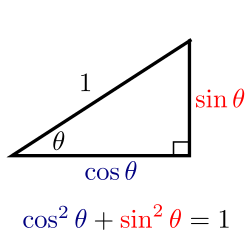
\includegraphics[scale=0.5]{Pythagorean}
\end{center}
By looking at a right triangle with hypotenuse 1 and angle $\theta$, and labeling the adjacent and opposite sides accordingly, one finds by using Pythagoras' Theorem that ${\cos^2 \theta + \sin^2 \theta = 1}$.\\
Another way to think about it is to embed the above triangle into a diagram for the unit circle where we see that ${\cos\theta}$ and ${\sin\theta}$ returns the x and y coordinates, respectively, of a point on the unit circle with angle $\theta$ to the $x$-axis:
\begin{center}
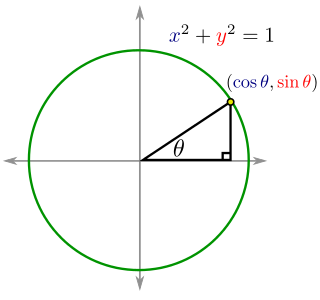
\includegraphics[scale=0.5]{UnitCircle}
\end{center}
That explains the nature of the formula ${\cos^{2} \theta+\sin^{2} \theta=1}$. It comes from the equation of the unit circle ${x^2 + y^2 = 1}$.\\
Others trigonometric functions:\\
${\tan=\displaystyle\frac{\sin}{\cos}}$\\
${\cot=\displaystyle\frac{\cos}{\sin}}$ , the reciprocal of $\tan$\\
${\sec=\displaystyle\frac{1}{\cos}}$ , the reciprocal of the $\cos$\\
${\csc=\displaystyle\frac{1}{\sin}}$ , the reciprocal of the $\sin$\\\\
All four of these have vertical asymptotes at the points where the denominator goes to zero.\\\\
\textbf{Inverse Trigonometrics}\\
We often write ${\sin^{-1}}$ to denote the inverse, but this can cause confusion. Be careful that ${\sin^{-1}\neq\displaystyle\frac{1}{\sin}}$. To avoid the confusion, the terminology $\arcsin$ is recommended for the inverse of the $\sin$ function.\\
The $\arcsin$ function takes on values ${\left[-\displaystyle\frac{\pi}{2},\frac{\pi}{2}\right]}$ and has a restricted domain ${\left[-1,1\right]}$.\\
The $\arccos$ function likewise has a restricted domain ${\left[-1,1\right]}$, but it takes values ${\left[0,\pi\right]}$.\\
The $\arctan$ function has an unbounded domain, it is well defined for all inputs. But it has a restricted range ${\displaystyle\left(-\frac{\pi}{2},\frac{\pi}{2}\right)}$.\\\\
\textbf{Exponentials}\\
Exponential functions are of the form ${c^x}$, where $c$ is some positive constant. The most common such function, referred to as \textit{the} exponential, is ${e^x}$. This is the most common because of its nice integral and differential properties (below).\\
Algebraic properties of the exponential function:\\
\begin{equation*} \displaystyle e^{x}e^{y}=e^{x+y} \end{equation*}
\begin{equation*} \displaystyle (e^{x})^{y}=e^{xy} \end{equation*}
Differential/integral properties:\\
\begin{equation*} \displaystyle\frac{d}{dx} e^{x}=e^{x} \end{equation*}
\begin{equation*} \displaystyle\int e^{x}dx=e^{x}+C \end{equation*}
Recall the graph of ${e^x}$, plotted here alongside its inverse, ${\ln x}$:\\
\begin{center}
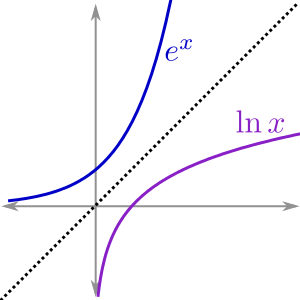
\includegraphics[scale=0.5]{ExpLn}
\end{center}
Note that the graphs are symmetric about the line ${y = x}$ (as is true of the graphs of a function and its inverse).\\
Before continuing, one might ask, what is $e$? There are several ways to define $e$, which will be revealed soon. For now, it is an irrational number which is approximately 2.718281828.\\\\
\textbf{Euler's Formula}\\
To close this lesson, we give a wonderful formula, which for now we will just take as a fact:\\
\begin{tcolorbox}
Euler's Formula
\begin{equation*} e^{ix}=\cos x+i\sin x \end{equation*}
\end{tcolorbox}
The $i$ in the exponent is the imaginary number ${\sqrt{-1}}$. It has the properties ${i^{2}=-1}$. $i$ is not a real number. That doesn't mean that it doesn't exist. It just means it is not on a real number line.\\
Euler's formula concerns the exponentiation of an imaginary variable. What exactly does that mean? How is this related to trigonometric functions? This will be covered in our next lesson.\\\\
\textbf{Additional Examples}\\\\
\textbf{Example:}\\
Find the domain of \[ f(x) = \frac{1}{\sqrt{x^2 -3x+2}}. \]
Answer:\\
te that the square root is only defined when its input is non-negative. Also, the denominator in a rational function cannot be 0. So we find that this function is well-defined if and only if ${x^2-3x+2>0}$. Factoring gives \[ (x-2)(x-1) > 0. \]
By plotting the points ${x=1}$ and ${x=2}$ (where the denominator equals 0) and testing points between them, one finds that ${x^2-3x+2>0}$ when ${x<1}$ or ${x>2}$:
\begin{center}
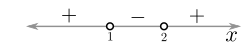
\includegraphics[scale=0.5]{PointChecking}
\end{center}
So the domain of $f$ is ${x<1}$ or ${2<x}$. In interval notation, this is ${\left(-\infty,1\right) \cup \left(2, \infty \right)}$.\\\\
\textbf{Example:}\\
Find the domain of \[ f(x) = \ln(x^3-6x^2+8x). \]
Answer:\\
Since $\ln$ is only defined on the positive real numbers, we must have ${x^3-6x^2+8x>0}$. Factoring gives \[ x(x^2-6x+8) = x(x-2)(x-4)>0 \]
As in the above example, plotting the points where this equals 0 and then testing points, we find that the domain is ${0<x<2}$ and ${4<x}$. In interval notation, this is ${\left(0,2 \right) \cup \left(4,\infty\right)}$.

\section{The Exponential} \label{ChFunctionsSecTheExponential}

This module deals with a very important function: the exponential. The first question one might ask is: what is the exponential function ${e^x}$? We know certain values of the function such as ${e^0=1}$, but what about an irrational input such as ${e^\pi}$, or an imaginary input ${e^i}$? Is it possible to make sense of these values?\\
The following definition answers these questions.\\
\begin{tcolorbox}
The Exponential $e^x$
\begin{align*} 
e^x &= 1+x+\frac{x^2}{2!} + \frac{x^3}{3!} + \frac{x^4}{4!} + \dotsb 
& = \sum_{k=0}^\infty \frac{x^k}{k!}, 
\end{align*}
where \[ k! = k(k-1)(k-2)\dotsb 3 \cdot 2 \cdot 1, \] and ${0! = 1}$
\end{tcolorbox}
One can now plug values for $x$ into the above sum to compute ${e^x}$. When ${x=0}$, for instance, one finds that ${e^0=1}$, (since all the terms with $x$ disappear) as expected. By plugging in ${x=1}$, the true value of $e$ is found to be ${e=1+1+\frac{1}{2!}+\frac{1}{3!}+\dotsb}$.\\\\

\subsection{A long polynomial}

There are technical concerns when trying to add up an infinite number of things. These issues will be dealt with later in the modules on \hyperref[ChDiscretizationSecSeries]{series}. For now, treat the infinite sum above as a long polynomial (the actual term is the Taylor series about ${x=0}$, which will be more formally dealt with in the \hyperref[ChFunctionsSecTaylorSeries]{next module}). Polynomials are nice because they are easy to integrate and differentiate. Recall the power rule for differentiating and integrating a monomial ${x^k}$, where $k$ is a constant:
\begin{align*}
\frac{d}{dx} x^k &= kx^{k-1} 
\int x^k \, dx &= \frac{1}{k+1} x^{k+1} + C \quad (k \neq -1) 
\end{align*}

\subsection{Properties of $e^x$}

Recall the following properties of the exponential function:
\begin{enumerate}
\item ${e^{x+y} = e^xe^y}$
\item ${e^{x\cdot y}=(e^x)^y=(e^y)^x}$
\item ${\frac{d}{dx}e^x = e^x}$
\item ${\int e^x dx=e^x+C}$.
\end{enumerate}
Consider the last two properties in terms of the long polynomial.Taking the derivative of the long polynomial for ${e^x}$ gives
\begin{align*} 
\frac{d}{dx}(1+x+\frac{x^2}{2!}+\frac{x^3}{3!} + \frac{x^4}{4!} + \dotsb)
&= 0 + 1 + \frac{2x}{2!} + \frac{3x^2}{3!} + \frac{4 x^3}{4!} + \dotsb\\
&= 1 + x + \frac{x^2}{2!} + \frac{x^3}{3!} + \dotsb,
\end{align*}
which is the original long polynomial. Integrating also gives (up to the constant of integration) the original long polynomial. This agrees with facts about the derivative and integral of ${e^x}$. Thus, the long polynomial for ${e^x}$ captures two of the key features of ${e^x}$; namely, ${e^x}$ is its own derivative and its own integral.

\subsection{Euler's formula}

Recall that the imaginary number $i$ is defined by ${i=\sqrt{-1}}$. So ${i^2=-1}$, ${i^3=-i}$, ${i^4=1}$, and this continues cyclically (for a review of complex/imaginary numbers, see \href{https://en.wikipedia.org/wiki/Complex_number}{wikipedia}). Assume the following fact, known as Euler's formula, mentioned in the last module.
\begin{tcolorbox}
	Euler's formula
	\begin{equation*} e^{ix} = \cos x + i \sin x. \end{equation*}
\end{tcolorbox}
Consider what happens when $ix$ is plugged into the long polynomial for ${e^x}$. By simplifying the powers of $i$, and grouping the result into its real and imaginary parts, one finds
\begin{align*} 
e^{ix} &= 1+ix+\frac{(ix)^2}{2!}+\frac{(ix)^3}{3!} + \dotsb\\
&= 1 + ix + \frac{i^2 x^2}{2!} + \frac{i^3 x^3}{3!} + \dotsb\\
&= 1 + ix - \frac{x^2}{2!} - i\frac{x^3}{3!} + \frac{x^4}{4!} + i \frac{x^5}{5!} + \dotsb\\
&= \left(1 - \frac{x^2}{2!} + \frac{x^4}{4!} - \dotsb\right) + i \left(x - \frac{x^3}{3!} + \frac{x^5}{5!} - \dotsb \right).
\end{align*}
If this is supposed to equal ${\cos x + i \sin x}$, then the real part must be ${\cos x}$, and the imaginary part must be ${\sin x}$. It follows that
\begin{align*}
\cos x &= 1 - \frac{x^2}{2!} + \frac{x^4}{4!} - \frac{x^6}{6!} + \dotsb = \sum_{k=0}^\infty (-1)^k \frac{x^{2k}}{(2k)!} \\
\sin x &= x - \frac{x^3}{3!} + \frac{x^5}{5!} - \frac{x^7}{7!} + \dotsb = \sum_{k=0}^\infty (-1)^k \frac{x^{2k+1}}{(2k+1)!}.
\end{align*}
These formulas should be memorized, both in their long polynomial form and their more concise summation notation form.\\\\
\textbf{Example:}\\
Compute ${1-\frac{\pi^2}{2!}+\frac{\pi^4}{4!}-\dotsb}$.\\
Answer:\\
Note that this is the long polynomial for ${\cos x}$, evaluated at ${x=\pi}$. So the value is ${\cos \pi = -1}$.\\\\
\textbf{Example:}\\
Check that taking the derivative of the long polynomial for ${\sin x}$ gives the long polynomial for ${\cos x}$ (hence, verify that ${\frac{d}{dx} \sin x = \cos x}$.\\
Answer:\\
Computing the derivative term by term gives
\begin{align*}
\frac{d}{dx} \sin(x) &= \frac{d}{dx} \left(x - \frac{x^3}{3!} + \frac{x^5}{5!} - \ldots \right) \\
&= 1 - 3 \frac{x^2}{3!} + 5 \frac{x^4}{5!} - \ldots \\
&= 1 - \frac{x^2}{2!} + \frac{x^4}{4!} - \ldots,
\end{align*}
which is the long polynomial for ${\cos x}$, as desired.\\\\
\textbf{Example:}\\
Show that the long polynomial for ${e^x}$ satisfies the first property above, namely ${e^{x+y} = e^x e^y}$. Hint: start with the long polynomials for ${e^x}$ and ${e^y}$ and multiply these together, and carefully collect like terms to show it equals the long polynomial for ${e^{x+y}}$.\\
Answer:\\
Beginning with ${e^x \cdot e^y}$, we find
\begin{align*}
e^x \cdot e^y &= \left(1+ x + \frac{x^2}{2!} + \dotsb \right) \left(1 + y + \frac{y^2}{2!} + \dotsb \right) \\
&= 1 + (x+y) + \left( \frac{x^2}{2!} + xy + \frac{y^2}{2!} \right) + \dotsb \\
&= 1 + (x+y) + \frac{x^2 + 2xy + y^2}{2!} + \dotsb \\
&= 1 + (x+y) + \frac{(x+y)^2}{2!} + \dotsb,
\end{align*}
which is the long polynomial for ${e^{x+y}}$, as desired.

\subsection{More on the long polynomial}

The idea of a long polynomial is reasonable, because it actually comes from taking a sequence of polynomials with higher and higher degree:
\begin{align*} 
f_0(x) &= 1 \\
f_1(x) &= 1+x \\
f_2(x) &= 1+x+\frac{x^2}{2} \\
f_3(x) &= 1+ x+ \frac{x^2}{2} + \frac{x^3}{6} \\
&\vdots. 
\end{align*}
Each polynomial in the sequence is, in a sense, the best approximation possible of that degree. Put another way, taking the first several terms of the long polynomial gives a good polynomial approximation of the function. The more terms included, the better the approximation. This is how calculators compute the exponential function (without having to add up infinitely many things).
\begin{center}
	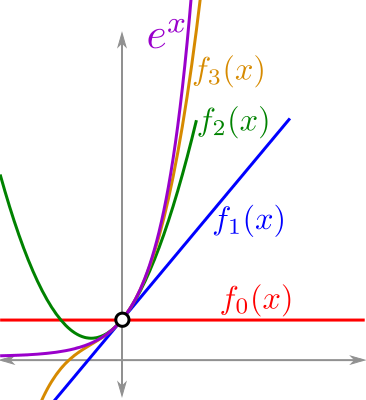
\includegraphics[scale=0.5]{ExponentialApproximants}
\end{center}
\noindent\makebox[\linewidth]{\rule{\paperwidth}{0.4pt}}

\subsection{Exercises}
\begin{itemize}
	\item So, how good of an approximation is a polynomial truncation of ${e^x}$? Use a calculator to compare how close $e$ is to the linear, quadratic, cubic, quartic, and quintic approximations. How many digits of accuracy do you seem to be gaining with each additional term in the series?
	\item Now, do the same thing with ${1/e}$ by plugging in ${x=-1}$ into the series. Do you have the same results? Are you surprised?
	\item Use the first three terms of the series for ${e^x}$ to approximate ${\sqrt[10]{e}}$ and ${e^{10}}$. How accurate do you think these approximations are?
	\item Calculate the following sum using what you know: \[\sum_{n=0}^\infty (-1)^n\frac{(\ln 3)^n}{n!}\]
	\item Write out the first four terms of the following series \[\sum_{n=0}^\infty (-1)^n\frac{\pi^{2n}}{2^n n!}\]
	\item Write out the following series using summation notation:\[1-\frac{2}{3!}+\frac{4}{5!}-\frac{8}{7!}+\cdots\]
	\item Estimate ${\sin(1/2)}$ to three digits of accuracy. How many terms in the series did this take?
	\item We've seen that ${i=e^{i\pi/2}}$ via Euler's formula. Using this and some algebra, tell me what is ${i^i}$. Isn't that nice? Now, tell me, what is ($(i^i)^i$)? Are you surprised? That's like, unreal!
	\item Practice your summation notation by rewriting the sum \[\sum_{n=2}^\infty (-1)^n\frac{x^{n-2}}{n^3}\] as a sum over an index that goes from zero to infinity.
	\item Use the first two nonzero terms of the Taylor series for ${\cos(x)}$ to approximate ${\cos(\frac{1}{10})}$.
	\item Use Euler's formula to derive the double angle formulas ${\cos(2\theta)=\cos^2(\theta)-\sin^2(\theta)}$ and ${\sin(2\theta)=2\sin(\theta)\cos(\theta)}$.
\end{itemize}

\section{Taylor series} \label{ChFunctionsSecTaylorSeries}
The long polynomial from the last module is actually called a Taylor series about ${x=0}$ (this is referred to as a Maclaurin series in some textbooks, but this course will use the term Taylor series). The last module gave the Taylor series for ${e^x}$, ${\sin x}$, and ${\cos x}$. The logical next question is to ask whether every function has a Taylor series.\\
The answer is that most \textit{reasonable} functions, and almost all of the functions encountered in this course, have a Taylor series. That is, every reasonable function $f$ can be written as \[f(x)=\sum_{k=0}^\infty c_k x^k=c_0+c_1 x+c_2 x^2+\dotsb.\]
This module describes how to compute the coefficients $c_k$ for a given function $f$.

\subsection{The definition of a Taylor series at x=0}
The definition of the Taylor series of $f$ at ${x=0}$ is
\begin{tcolorbox}
	Taylor series at ${x=0}$
	\begin{equation*}	
	f(x) = f(0) + \frac{f'(0)}{1!}x + \frac{f(0)}{2!}x^2 + \frac{f'(0)}{3!}x^3+\dotsb = \sum_{k=0}^\infty \frac{f^{\left(k\right)}(0)}{k!} x^k,
	\end{equation*}
	where ${f^{\left(k\right)}(0)}$ is the $k$th derivative of $f$ evaluated at 0. In other words, the coefficient $c_k$ mentioned above is given by \[c_k=\frac{f^{\left(k\right)}(0)}{k!}=\frac{1}{k!}\cdot\frac{d^k f}{dx^k}\bigg|_0\] 
\end{tcolorbox}
This seems circular, since the definition uses the function, and its derivatives, to write down the function. However, the definition only actually requires information about the function at a single point (in this case, 0). It is best to think of the Taylor series as a way of turning a function into a polynomial.\\
\textbf{Example} Compute the Taylor series for $e^x$ using the above definition to see that it matches the given series from the last module.\\
Answer:\\
Here, ${f(x)=e^x}$, and every derivative of $e^x$ is $e^x$. Therefore, for all $k$ we have \[f^{\left(k\right)}(x)=e^x,\] and so ${f^{\left(k\right)}(0)=1}$ for all $k$. Plugging into the Taylor series formula gives
\begin{align*}
f(x) &= \sum_{k=0}^\infty \frac{f^{\left(k\right)}(0)}{k!} x^k \\
&= \sum_{k=0}^\infty \frac{x^k}{k!} \\
&= 1 + x + \frac{x^2}{2!} + \frac{x^3}{3!} + \dotsb, 
\end{align*}
as claimed.\\\\
\textbf{Example} Compute the Taylor series for ${f(x)=\sin x}$ using the above definition, and verify it matches the series found using Euler's formula.\\
Answer:\\
Computing the derivatives, and then evaluating at ${x=0}$ gives the following table:
\begin{align*}
f(x) &= \sin(x) & f(0) &= 0 \\
f'(x) &= \cos(x) & f'(0) &= 1 \\
f''(x) &= -\sin(x) & f''(0) &= 0 \\
f'''(x) &= -\cos(x) & f'''(0) &= -1 \\
& \vdots 
\end{align*}
Thus,
\begin{align*}
\sin(x) &= 0+\frac{1}{1!}x+\frac{0}{2!}x^2+\frac{-1}{3!}x^3+\dotsb \\
&= x - \frac{x^3}{3!} + \frac{x^5}{5!} - \dotsb,
\end{align*}
confirming what was found last time.\\\\
\textbf{Example} Compute the Taylor series for ${f(x) = x^2-5x+3}$.\\
Again, by directly using the definition:
\begin{align*}
f(x) &= x^2-5x+3 & f(0) &= 3 \\
f'(x) &= 2x-5 & f'(0) &= -5 \\
f''(x) &= 2 & f''(0) &= 2 \\
f'''(x) &= 0 & f'''(0) &= 0 \\
& \vdots
\end{align*}
So it follows that \[f(x)=3-5x+\frac{2}{2!}x^2=3-5x+x^2\]
(since all the subsequent derivatives are 0), which is the original function. This should not be a surprise, since the Taylor series represents a function as a long polynomial (henceforth called by its proper name: \textit{series}). If $f$ was a polynomial to begin with, it stands to reason that the Taylor series for $f$ should just be $f$ itself.

\subsection{Why Taylor series matter}
The big idea of this module is that the Taylor series can be thought of as an operator (a machine) which turns a function into a series. This is a useful operator because some functions are hard (or even impossible) to express using combinations of familiar functions. Nevertheless, these functions can often be understood by computing their Taylor series.\\
\textbf{Example} The \textit{Bessel function}, denoted $J_0$, is best defined by its Taylor series:
\begin{align*} 
J_0 &= \sum_{k=0}^\infty (-1)^k \frac{x^{2k}}{2^{2k} (k!)^2} \\
&= 1 - \frac{1}{2^2} x^2 + \frac{1}{2^4(2!)^2}x^4 - \frac{1}{2^6 (3!)^2}x^6 + \dotsb 
\end{align*}
This series has only the even powers of $x$, and it alternates, which is reminiscent of the series for cosine. One difference is that the denominator in the Bessel function grows more quickly than the denominator in the series for cosine. Thus, we might expect the graph to be a wave with a decreasing amplitude, which is exactly what we find:
\begin{center}
	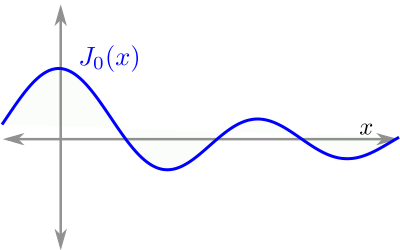
\includegraphics[scale=0.5]{Bessel}
\end{center}
It turns out that the Bessel function describes many physical phenomena, including the shape of a hanging chain as it is rotated, and the shape of the waves formed after a stone is thrown into a pool of water.

\subsection{Taylor series as polynomial approximants}
The main reason Taylor series are useful is that they turn a potentially complicated function into something simple: a polynomial. Granted, this polynomial is infinitely long in general, but in practice it is only necessary to compute the first few terms to get a good, local approximation of the function. The more terms one includes, the better the polynomial approximates the function.\\
As an example, consider a particle on the number line with position function $p(t)$. At time 0, say its position is 5. Then one approximation of its position as a function of time is ${p_0(t)=5}$. Given more information, say its velocity at time 0 is 3, the approximation becomes better. The next approximation as a function of time is ${p_1(t)=5+3t}$. Now, suppose its acceleration at time 0 is $-4$. Then ${p_2(t)=5+3t-\frac{4}{2}t^2=5+3t-2t^2}$ is an even better polynomial approximation of the position function.\\
\begin{center}
	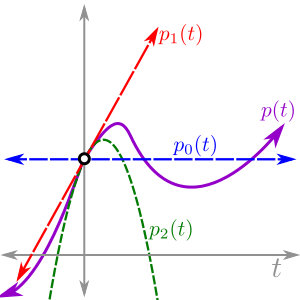
\includegraphics[scale=0.5]{Approximants}
\end{center}
\noindent\makebox[\linewidth]{\rule{\paperwidth}{0.4pt}}

\subsection{Exercises}
\begin{itemize}
\item What is the Taylor series of ${x^4-3x^3+2x^2+7x-3}$. This should be an easy one!
\item What is the Taylor series of ${(x-2)^2(x-3)}$? This, also, should not be *too* hard...
\item Compute a few derivatives and figure out the first few terms of the Taylor series of ${\displaystyle\frac{1}{1-x}}$. Have you seen this series before?
\item What are the first two nonzero terms in the Taylor series of ${\sqrt[3]{1-2x}}$?
\item What is the coefficient of the cubic term in the Taylor series of ${e^{-3x}}$?
\item Use what you know about Taylor series to determine the third derivative of ${\sin^3(2x)\cos^2(3x)}$ at ${x=0}$. That's a *lot* easier than computing the derivatives!
\item The ERF function is defined in terms of a difficult integral: \[ERF(x)=\frac{2}{\sqrt{\pi}}\int_0^x e^{-t^2}\,dt\]
\item Even if you don't remember integrals all that well, you know how to integrate a polynomial, right? So, Taylor expand the integrand and integrate term by term to get the Taylor series for ERF.
\item What is the third derivative of ERF(x) at zero?
\item Why does a Taylor series have all those ($n!$) terms in the denominator? Let's see. Compute the Taylor series of ${f(x)=(1+x)^5}$ by (1) using the binomial theorem (or multiplication) to expand that power; then (2) by differentiating the function and using the Taylor series formula. What do you notice when you keep computing higher derivatives?
\end{itemize}

\section{Computing Taylor series} \label{ChFunctionsSecComputingTaylorSeries}
The previous module gave the definition of the Taylor series for an arbitrary function. It turns out that this is not always the easiest way to compute a function's Taylor series. Just as functions can be added, subtracted, multiplied, and composed, so can their corresponding Taylor series.\\
Recall that the Taylor series for a function ($f$) is given by \[f(x)=\sum_{k=0}^\infty \frac{f^{\left(k\right)}(0)}{k!} x^k=f(0)+f'(0)x+\frac{f''(0)}{2!} x^2+\dotsb.\]
Using the definition of the Taylor series involves taking a lot of derivatives, which could be a lot of work, especially if the function involves compositions and products of functions, e.g. ${f(x)=\sin(x^2)e^{x^3}}$. This module will show how to compute the Taylor series of such functions more easily by using the Taylor series for functions we already know.

\subsection{Substitution}
Our first method, substitution, allows us to plug one function into the Taylor series of another. Consider the function \[f(x)=\frac{1}{x}\sin(x^2).\]
Computing the Taylor series for $f$ from the definition would involve the quotient rule, chain rule, and a lot of algebra. But by taking the series for ${\sin x}$ and substituting $x^2$ into this series, and then distributing the ${\frac{1}{x}}$, one finds
\begin{align*}
\frac{1}{x}\sin(x^2)&=\frac{1}{x}\left((x^2)-\frac{1}{3!}(x^2)^3+\frac{1}{5!}(x^2)^5-\dotsb\right) \\
&=\frac{1}{x}\left(x^2-\frac{1}{3!}x^6+\frac{1}{5!}x^{10}-\dotsb\right) \\
&=x-\frac{1}{3!}x^5+\frac{1}{5!}x^9-\dotsb. 
\end{align*}
Note that getting this many terms using the definition would involve taking nine derivatives of the original function, which would be a lot of work! To get a more complete description of the Taylor series, one can use the summation notation, and again substitute to find
\begin{align*}
\frac{1}{x} \sin(x^2) &= \frac{1}{x} \sum_{k=0}^\infty (-1)^k \frac{(x^2)^{2k+1}}{(2k+1)!} \\
&= \frac{1}{x} \sum_{k=0}^\infty (-1)^k \frac{x^{4k+2}}{(2k+1)!} \\
&= \sum_{k=0}^\infty (-1)^k \frac{x^{4k+1}}{(2k+1)!}
\end{align*}
\textbf{Example} Find the Taylor series for ${e^{x^3}}$ by substitution.\\
Answer:\\
Recall the series for $e^x$ is \[e^x=1+x+\frac{x^2}{2!}+\frac{x^3}{3!}+\dotsb=\sum_{k=0}^\infty\frac{x^k}{k!}\]
Substituting $x^3$ into the series for $e^x$ gives
\begin{align*}
e^{x^3} &= 1 + x^3 + \frac{(x^3)^2}{2!} + \frac{(x^3)^3}{3!} + \dotsb \\
&= 1 + x^3 + \frac{x^6}{2!} + \frac{x^9}{3!} + \dotsb \\
&= \sum_{k=0}^\infty \frac{(x^3)^k}{k!} \\
&= \sum_{k=0}^\infty \frac{x^{3k}}{k!}
\end{align*}

\subsection{Combining like terms}
Another way to use previous knowledge of one Taylor series to find another is by combining like terms. This requires some careful algebra, but it is no more difficult than multiplying two polynomials together. For example, consider the function \[f(x)=\cos^2(x)=\cos(x)\cdot\cos(x).\]
Finding the series for a function multiplied by another function is the same as taking the series for each function and multiplying them together, and then collecting like terms. This is where some algebra is required.
\begin{align*}
\cos(x)\cdot\cos(x)&=\left(1-\frac{1}{2!}x^2+\frac{1}{4!}x^4-\dotsb\right)\left(1-\frac{1}{2!}x^2+\frac{1}{4!}x^4-\dotsb\right) \\ 
&=1+\left(-\frac{1}{2!}-\frac{1}{2!}\right)x^2+\left(\frac{1}{4!}+\frac{1}{2!}\frac{1}{2!}+\frac{1}{4!}\right)x^4+\dotsb \\
&=1-x^2+\frac{1}{3}x^4+\dotsb.
\end{align*}
To see where the coefficient of $x^4$ comes from, note that every $x^4$ term comes from some term from the left series multiplied together with some term from the right series whose powers add up to 4. There are three such pairs: 1 on the left paired with ${\frac{1}{4!}x^4}$ on the right; ${-\frac{1}{2!}x^2}$ on the left paired with ${-\frac{1}{2!}x^2}$ on the right; and ${\frac{1}{4!}x^4}$ on the left paired with 1 on the right. This is the same algebra one would do when multiplying two polynomials together; this is just a way of collecting like terms in a systematic way.\\\\
\textbf{Example} Use the trigonometric identity \[\cos^2x=\frac{1+\cos(2x)}{2}\] and substitution to find the series for ${\cos^2x}$. Try to give the series in summation notation (other than the first term)\\
Answer:\\
By the above identity,
\begin{align*}
\cos^2x &= \frac{1}{2} \left(1 + \cos(2x)\right) \\
&= \frac{1}{2} \left(1 + \left(1 - \frac{(2x)^2}{2!} + \frac{(2x)^4}{4!} - \dotsb \right)\right) \\
&= \frac{1}{2} \left(2 - \frac{4x^2}{2} + \frac{16x^4}{24} - \dotsb \right) \\
&= 1 - x^2 + \frac{x^4}{3} - \dotsb.
\end{align*}
In summation notation,
\begin{align*}
\cos^2x &= \frac{1}{2} \left(1 + \sum_{k=0}^\infty (-1)^k \frac{(2x)^{2k}}{(2k)!}\right)  \\
&= \frac{1}{2} + \frac{1}{2} \sum_{k=0}^\infty (-1)^k \frac{(2x)^{2k}}{(2k)!} \\
&= \frac{1}{2} + \sum_{k=0}^\infty (-1)^k \frac{2^{2k-1}x^{2k}}{(2k)!} \\
&= 1 + \sum_{k=1}^\infty (-1)^k \frac{2^{2k-1}x^{2k}}{(2k)!}.
\end{align*}

\subsection{Hyperbolic trigonometric functions}
The hyperbolic trigonometric functions ${\sinh(x)}$, ${\cosh(x)}$, and ${\tanh(x)}$ are defined by
\begin{align*}
\sinh(x) &= \frac{e^x - e^{-x}}{2} \\
\cosh(x) &= \frac{e^x+e^{-x}}{2} \\
\tanh(x) &= \frac{e^x - e^{-x}}{e^x + e^{-x}} = \frac{\sinh(x)}{\cosh(x)}.
\end{align*}
\begin{center}
	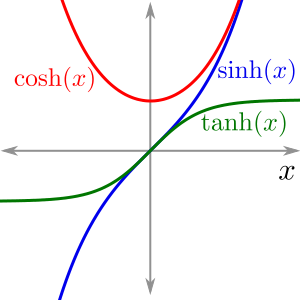
\includegraphics[scale=0.5]{Hyperbolic}
\end{center}
These hyperbolic trig functions, although graphically quite different from their traditional counterparts, have several similar algebraic properties, which is why they are so named. For example, the Pythagorean identity for cosine and sine has a version for hyperbolic cosine and sine: \[\cosh^2(x)-\sinh^2(x)=1.\]
One can verify this using the definitions and some algebra. But there is a geometric intuition for this relationship. Recall that cosine and sine give the $x$ and $y$ coordinates, respectively, for a point on the unit circle ${x^2+y^2=1}$. The hyperbolic cosine and hyperbolic sine give the $x$ and ($y$) coordinates, respectively, for points on the hyperbola ${x^2-y^2=1}$:
\begin{center}
	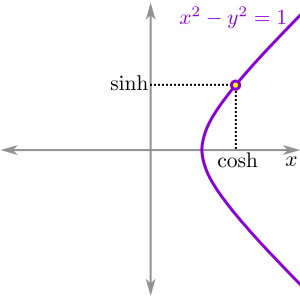
\includegraphics[scale=0.5]{HyperbolicPlot}
\end{center}
\textbf{Example} Using the Taylor series for $e^x$ and substitution, show that the Taylor series for $\cosh$ and $\sinh$ are
\begin{align*}
\cosh(x) &= 1 + \frac{x^2}{2!} + \frac{x^4}{4!} + \dotsb = \sum_{k=0}^\infty \frac{x^{2k}}{(2k)!} \\
\sinh(x) &= x + \frac{x^3}{3!} + \frac{x^5}{5!} + \dotsb = \sum_{k=0}^\infty \frac{x^{2k+1}}{(2k+1)!}. \end{align*}
Note that these are almost the same as the series for cosine and sine, respectively, except they do not alternate. This gives another reason for the names of these functions.\\
Answer:\\
\begin{align*}
\cosh(x) &= \frac{e^x + e^{-x}}{2} \\
&= \frac{1}{2}\left[(1+x+\frac{x^2}{2!} + \dotsb)+(1-x+\frac{x^2}{2!}-\dotsb)\right] \\
&= \frac{1}{2}\left[2 + 2 \frac{x^2}{2!} + 2 \frac{x^4}{4!} +\dotsb \right] \\
&= 1+\frac{x^2}{2!} + \frac{x^4}{4!}+\dotsb \\
&= \sum_{k=0}^\infty \frac{x^{2k}}{(2k)!}.
\end{align*}
\begin{align*}
\sinh(x) &= \frac{e^x - e^{-x}}{2} \\
&= \frac{1}{2}\left[(1+x+\frac{x^2}{2!} + \dotsb)-(1-x+\frac{x^2}{2!}-\dotsb)\right] \\
&= \frac{1}{2}\left[2x + 2 \frac{x^3}{3!} + 2 \frac{x^5}{5!} +\dotsb \right] \\
&= x+\frac{x^3}{3!} + \frac{x^5}{5!}+\dotsb \\
&= \sum_{k=0}^\infty \frac{x^{2k+1}}{(2k+1)!}.
\end{align*}

\subsection{Manipulating Taylor series}
Another way of using one Taylor series to find another is through differentiation and integration. For instance, to find the Taylor series for the derivative of $f$, one can differentiate the Taylor series for $f$ term by term.\\
\textbf{Example} By differentiating the Taylor series for $\sinh$ and $\cosh$, show that
\begin{align*}
\frac{d}{dx} \sinh x &= \cosh x \\
\frac{d}{dx} \cosh x &= \sinh x.
\end{align*}
This is yet another relationship which is similar (though not identical) to the relationship between sine and cosine.\\
Answer:\\
Differentiating hyperbolic sine gives
\begin{align*}
\frac{d}{dx}\sinh x &= \frac{d}{dx}\sum_{k=0}^\infty\frac{x^{2k+1}}{(2k+1)!} \\
&= \sum_{k=0}^\infty (2k+1) \frac{x^{2k}}{(2k+1)!} \\
&= \sum_{k=0}^\infty \frac{x^{2k}}{(2k)!} \\
&= \cosh x,
\end{align*}
as desired. Similarly, differentiating hyperbolic cosine gives
\begin{align*}
\frac{d}{dx}\cosh x &= \frac{d}{dx} \sum_{k=0}^\infty \frac{x^{2k}}{(2k)!} \\
&= \sum_{k=0}^\infty (2k) \frac{x^{2k-1}}{(2k)!} \\
&= \sum_{k=1}^\infty \frac{x^{2k-1}}{(2k-1)!} \\
&= \sum_{k=0}^\infty \frac{x^{2k+1}}{(2k+1)!}.
\end{align*}
There was a little bit of reindexing there, but by writing out a few terms of each series, one can see that all of the above equalities are true.

\subsection{Higher Order Terms in Taylor Series}
In some situations, it will be convenient only to write the first few terms of a Taylor series. This is particularly true when combining or composing more than one Taylor series. Up until now, an ellipsis has been used to indicate that there are more terms in the series that are being omitted.\\
There is another way, sometimes used in this course, of notating the omitted terms in a Taylor series. That is by referring to them as Higher Order Terms (or H.O.T. for short). Having the extra HOT in a series means that all the remaining terms in the series have a higher degree than the previous terms.\\\\
\textbf{Example} The function $e^x$ can be written as \[e^x=1+x+\frac{1}{2!}x^2+\hbox{ HOT},\] or it could also be written as \[e^x=1+x+\hbox{ HOT}.\]
The point at which the higher order terms are cut-off is somewhat arbitrary and depends on the situation. There is a more formal way of keeping track of the higher order terms, called Big-O notation, which is presented in \hyperref[ChFunctionsSecOrdersOfGrowth]{orders of growth}.\\\\
\textbf{Example} Find the first two non-zero terms of the Taylor series for \[f(x)=1-2xe^{\sin x^2}.\]
Answer:\\
Beginning with the innermost function, in this case ${\sin x^2}$, we find that \[\sin x^2=x^2-\frac{1}{3!}(x^2)^3+\hbox{HOT}=x^2-\frac{1}{6}x^6+\hbox{HOT}.\]
Then plugging this into the series for $e^x$ gives
\begin{align*}
e^{\sin x^2}&=1+\left(x^2-\frac{1}{6}x^6+\hbox{HOT}\right)+\frac{1}{2!}\left(x^2+\hbox{HOT}\right)^2+\frac{1}{3!}\left(x^2+\hbox{HOT}\right)^3+\hbox{HOT} \\
&=1+x^2+\frac{1}{2}x^4+\left(-\frac{1}{6}+\frac{1}{6}\right)x^6+\hbox{HOT} \\
&=1+x^2+\frac{1}{2}x^4+\hbox{HOT}
\end{align*}
Then to complete the answer, plug this into the original function to find
\begin{align*}
f(x) &= 1 - 2x \left( 1 + x^2 + \frac{1}{2}x^4 + \hbox{ HOT}\right) \\
&= 1 - 2x - 2x^3 - x^5 + \hbox{ HOT}.
\end{align*}

\subsection{Extra examples}
\textbf{Example}\\
Compute the Taylor series (at 0) for ${\sin^2 x}$ up to and including terms of order 6. Try to give the full Taylor series in summation notation.\\
Answer:\\
\begin{align*}
\sin^2 x &= (x-\frac{x^3}{3!}+\frac{x^5}{5!}-\dotsb)(x-\frac{x^3}{3!}+\frac{x^5}{5!}-\dotsb) \\
&=x^2+(-\frac{1}{3!}-\frac{1}{3!})x^4+(\frac{1}{5!}+\frac{1}{3!\cdot 3!}+\frac{1}{5!})x^6+\dotsb \\
&= x^2-\frac{1}{3}x^4+\frac{2}{45}x^6-\dotsb.
\end{align*}
To get the full Taylor series, one can use the identity \[\sin^2 x=\frac{1-\cos(2x)}{2}\] to find that
\begin{align*}
\sin^2 x &= \frac{1-\cos(2x)}{2} \\
&=\frac{1}{2}\left(1-\left(1-\frac{(2x)^2}{2!}+\frac{(2x)^4}{4!}-\dotsb\right)\right) \\
&=\frac{1}{2}\left(\frac{(2x)^2}{2!}-\frac{(2x)^4}{4!}+\frac{(2x)^6}{6!}-\dotsb\right) \\
&=\frac{1}{2}\sum_{k=1}^\infty(-1)^{k-1}\frac{(2x)^{2k}}{(2k)!}.
\end{align*}
\\\textbf{Example}\\
Find the first three terms of the Taylor series for ${\sqrt{f(x)}}$, where \[f(x)=a_0+a_1 x+a_2 x^2+a_3x^3+\dotsb.\]
Answer:\\
Let ${g(x)=\sqrt{f(x)}}$), where \[g(x)=b_0+b_1 x+b_2 x^2+b_3 x^3+\dotsb.\]
Then ${g(x)^2=f(x)}$, and so the same holds for the Taylor series: \[\left(b_0+b_1 x+b_2 x^2+b_3 x^3+\dotsb\right)^2=a_0+a_1 x+a_2 x^2+\dotsb.\]
Multiplying out and collecting like terms gives \[b_0^2+(b_0b_1+b_1b_0)x+(b_0b_2+b_1b_1+b_2b_0) x^2+\dotsb=a_0+a_1 x+a_2 x^2+\dotsb.\]
Now, equating coefficients of the monomials on the left and right gives the first few equations (of an infinite system of equations)
\begin{align*}
b_0^2 &= a_0 \\ 
2b_0b_1 &= a_1 \\
2b_0b_2 + b_1^2 &= a_2.
\end{align*}
Solving these equations gives the first three coefficients of $g$:
\begin{align*}
b_0 &= \sqrt{a_0} \\
b_1 &= \frac{a_1}{2 \sqrt{a_0}} \\
b_2 &= \frac{1}{2\sqrt{a_0}}\left(a_2-\frac{a_1^2}{4a_0}\right).
\end{align*}
Thus, \[\sqrt{a_0+a_1 x+a_2 x^2+\dotsb}=\sqrt{a_0}+\frac{a_1}{2\sqrt{a_0}}x+\frac{1}{2\sqrt{a_0}}\left(a_2-\frac{a_1^2}{4a_0}\right)x^2+\dotsb.\]

\subsection{Exercises}
\begin{itemize}
\item Compute the Taylor series of ${\cos(2x)\sin(3x)}$ up to and including terms of degree 5. Don't try computing derivatives for this!
\item Use a Taylor polynomial to give a cubic approximation to ${2xe^{3x}}$
\item Compute the Taylor series of ${e^{1-\cos t}}$ in summation notation.
\item Compute the Taylor series of ${\cos(\sin(x))}$ to fourth order.
\item Compute the Taylor series of ${\sin(\cos(x))}$ to forth order. What happens that makes this different than the last problem? (Hint: ${\cos(0)=1}$ but ${\sin(0)=0}$...)
\item Compute the first three nonvanishing terms in the Taylor series of ${e^{2x}(\sinh 3x)/x}$.
\item Compute the Taylor series of ${3x^2 e^{-x^2} \sin 2x^3}$ up to and including terms of order eight! Wow, that means a lot of work, right? Think... which terms should you expand first?
\item Compute the Taylor series of ${\frac{1}{x}e^{-x^2}\sinh(2x)}$ up to the fourth order term.
\item What is the second derivative of the function ${e^{x\cosh(x^2)}}$ at ${x=0}$?
\item Compute the following limit ${\lim_{x\to0}(1-e^x)\frac{\sin(x^2)}{x^3}}$
\end{itemize}

\section{Convergence} \label{ChFunctionsSecConvergence}
\section{Expansion points} \label{ChFunctionsSecExpansionPoints}
\section{Limits} \label{ChFunctionsSecLimits}
\section{L'Hopital's Rule} \label{ChFunctionsSecLHopitalsRule}
\section{Orders of growth} \label{ChFunctionsSecOrdersOfGrowth}

\chapter{Differentiation} \label{ChDifferentiation}
\section{Derivatives} \label{ChDifferentiationSecDerivatives}
\section{Differentiation rules} \label{ChDifferentiationSecDifferentiationRules}
\section{Linearization} \label{ChDifferentiationSecLinearization}
\section{Higher derivatives} \label{ChDifferentiationSecHigherDerivatives}
\section{Optimization} \label{ChDifferentiationSecOptimization}
\section{Differentials} \label{ChDifferentiationSecDifferentials}
\section{Differentiation as an operator} \label{ChDifferentiationSecDifferentiationAsAnOperator}

\chapter{Integration} \label{ChIntegration}
\section{Antidifferentiation} \label{ChIntegrationSecAntidifferentiation}
\section{Exponential growth examples} \label{ChIntegrationSecExponentialGrowthExamples}
\section{More differential equations} \label{ChIntegrationSecMoreDifferentialEquations}
\section{ODE Linearization} \label{ChIntegrationSecODELinearization}
\section{Integration by Substitution} \label{ChIntegrationSecIntegrationBySubstitution}
\section{Integration by parts} \label{ChIntegrationSecIntegrationByParts}
\section{Trigonometric substitution} \label{ChIntegrationSecTrigonometricSubstitution}
\section{Partial fractions} \label{ChIntegrationSecPartialFractions}
\section{Definite integrals} \label{ChIntegrationSecDefiniteIntegrals}
\section{Fundamental Theorem of Integral Calculus} \label{ChIntegrationSecFundamentalTheoremOfIntegralCalculus}
\section{Improper integrals} \label{ChIntegrationSecImproperIntegrals}
\section{Trigonometric integrals} \label{ChIntegrationSecTrigonometricIntegrals}
\section{Tables and computers} \label{ChIntegrationSecTablesAndComputers}

\chapter{Applications} \label{ChApplications}

\chapter{Discretization} \label{ChDiscretization}
\section{Series} \label{ChDiscretizationSecSeries}

\end{sloppypar}
\end{document}
